\chapter{Levantamento Bibliográfico}\label{cap:levbibliog}

Este capítulo apresenta uma breve introdução à Smart Cities, Crowdsourcing, contexto atual do desenvolvimento de programação voltada a aplicativos de transporte público e demais conceitos, pormenores, ao desenvolvimento do trabalho.

\section{Smart Cities}

O conceito de Cidades Inteligentes e o respectivo aumento no seu uso, pode ser reconhecido como o resultado do alto crescimento das tecnologias digitais na intenção de garantir um futuro sustentável. Embora o conceito seja empregado normalmente com o objetivo de elaborar estratégias que objetivem melhorar a qualidade de vida dos cidadãos, criando um futuro sustentável, o conceito por si só continua sendo usado em diferentes contextos e assim permanece um tanto ambíguo. Dessa forma faz-se necessário estabelecer um critério muito importante que o diferencia das cidades-conceito, o aspecto colaborativo entre os diversos interessados, mais comumente os cidadãos \cite{schuurman}. 

Um outro enfoque, mais empresarial, apresentado por \citeonline{walravens}, menciona que o conceito também pode ser empregado para caracterizar um grupo de organizações que intentam por revolucionar algum aspecto em uma região, entre os quais estão parques empresariais, o nível de escolaridade de uma população, o uso de tecnologias em contextos urbanos, o aumento da eficácia de governos e especialmente aquelas com foco em ITC. Walravens argumenta também que de maneira geral, o uso de serviços de telefonia móvel adquirem uma importância inevitável, já que é um sub aspecto de ITC e dessa forma grande importância na construção de uma Cidade Inteligente \cite{walravens}.

Em vista disso, sistemas operacionais desenvolvidos para \emph{smartphones} inspiram desenvolvedores a conceber aplicativos e serviços que aperfeiçoam a vida nas cidades de diversas formas diferentes, como por exemplo, facilitando acesso à informação sobre o transporte publico. Além disto, à medida que os \emph{smartphones} se tornam mais acessíveis e populares, cria-se o desejo de que se tornem eminentes ferramentas na busca de uma cidade mais inteligente \cite{walravens}.




%A fundamentação teórica atribui, essencialmente, credibilidade ao trabalho, faz referência às pesquisas e aos conhecimentos já construídos e publicados, situando a evolução do assunto e, assim, dando sustentação ao tema que está sendo estudado.

%É preciso situar historicamente a evolução do tema, quais as abordagens já investigadas, qual o estágio atual do conhecimento sobre o assunto ou quais as tendências que se apresentam.

%É necessário apresentar uma análise do estado da arte do problema abordado. Não se trata de uma simples transcrição de pequenos textos ou citações, mas sim de uma sistematização de ideias, fundamentos, conceitos e proposições de vários autores, apresentados de forma lógica, encadeada e descritiva, demonstrando que foram estudados e analisados pelo autor.

%Deve-se realizar o levantamento bibliográfico junto a diferentes fontes documentais, como livros, obras de referência, periódicos científicos, teses, dissertações, monografias, artigos, dentre outros.

%inicio

%Um aplicativo que aproxima-se bastante do projeto proposto é o chamado ``Waze''. O aplicativo foi comprado pela Google em 2013 por cerca de US$\$$ 1,3 bilhões. Cohan aponta quatro grandes motivos para a compra do aplicativo pela Google.

%Segundo Cohan, um dos motivos é o compromisso que um usuário adquire ao utilizar o Waze. A comunidade de usuários beira os 50 milhões; são 50 milhões de usuários contribuindo com informações sobre o trânsito, em praticamente qualquer local do planeta, à todo momento. A comunidade atribui espécies de ``recompensas'', através de pontuações e insígnias, à usuários que realmente são comprometidos em ajudar os outros (COHAN). A Google pode aproveitar esse esquema de comunidades de usuários e \emph{crowdsourcing} para aplicar em futuros projetos. 

%Outro fator importante é que o Waze acaba sendo um complemento ao serviço Google Maps, bastante popular. O aplicativo permite que usuários notifiquem os outros sobre acidentes, radares e ruas bloqueadas, por exemplo, através da utilização de \emph{crowdsourcing}. Para Cohan, o Waze apresenta-se não apenas como um complemento, mas também uma alternativa ao tradicional Google Maps. 

%(TODO: INCLUIR FONTE DO COHAN http://www.forbes.com/sites/petercohan/2013/06/11/four-reasons-for-google-to-buy-waze/)

%(TODO: DESCREVER FUNCIONAMENTO DO WAZE)

\section{Crowdsourcing}

Outro aspecto importante  a ser mencionado é a caracterização de \emph{crowdsourcing}, no que tange inteligência coletiva. À grosso modo, entende-se inteligência coletiva como quando indivíduos de um determinado grupo, que possui interesse por determinado assunto, combinam seus conhecimentos a fim de encontrar a solução para um determinado problema.  Através da interação social, o conhecimento individual é compartilhado, corrigido, processado, enriquecido e avaliado. Normalmente, os resultados colhidos são melhores que os obtidos por um único indivíduo. Talvez a aplicação mais difundida desse conceito seja a Wikipedia  \cite{schuurman}. 

Por conseguinte, a ponte que se estabelece entre \emph{crowdsourcing} e \emph{smart cities} acompanha o advento dos smartfones. Para \citeonline{kanhere}, as melhorias no poder de processamento, sensoriamento e capacidades de armazenamento permite que telefones celulares sejam comparados a dispositivos de computação. Esse fenômeno abre margem ao surgimento de um novo paradigma, denominado pela literatura de sensoriamento participativo, cuja ideia principal gira em torno de capacitar um cidadão comum a coletar e compartilhar dados de sensoriamento do ambiente em que está inserido, a partir de seu telefone celular \cite{kanhere}.

Ainda segundo Kanhere, sensoriamento participativo possui quatro vantagens principais sobre redes de sensores tradicionais (já que esta necessita de uma gama considerável de dispositivos sem fio, principalmente em áreas urbanizadas), sendo elas: custo de implementação baixo, já que usa telefones celulares e Wi-Fi; uma ampla mobilidade e cobertura proporcionada pelas operadoras de telefonia; economias de escala proporcionadas pelo uso de celulares; a facilidade assegurada pelas lojas de aplicativos e também as inúmeras formas de desenvolvimento de software disponíveis para sistemas operacionais de dispositivos móveis \cite{kanhere}. 

Com base em todos esses conceitos, estabelece-se, a seguir, um breve estado da arte registrado na literatura, no que se refere à área de desenvolvimento de aplicativos para plataformas móveis dentro da ideia de \emph{crowdsourcing} e \emph{smart cities}.

\section{Estado da Arte}

Conforme já relacionado na Introdução, \citeonline{sujatha} propuseram um sistema chamado MBTS para que qualquer pessoa obtenha informações de um determinado ônibus através de um aplicativo móvel. 

Três são os atores do sistema: os passageiros, os chamados ``coordenadores'' do ônibus e as pessoas que estão aguardando em um ponto. Todos os atores necessitam de um \textit{smartphone} com sistema operacional Android conectado à Internet. Continuamente, os passageiros e os ``coordenadores'' alimentam um banco de dados com informações sobre o ônibus. Essas informações podem ser as coordenadas do ônibus, obtidas através do GPS integrado ao \emph{smartphone}, ou até mesmo a ``situação'' do ônibus -- se ele está lotado ou vazio, se houve algum acidente, se o ônibus está atrasado, entre outros. Essas informações ficam armazenadas em um banco de dados para serem acessadas, posteriormente, por alguém que esteja utilizando o aplicativo, principalmente usuários que estão aguardando um ônibus em algum ponto. 

%Em linhas gerais, os objetivos do MBTS são os seguintes \cite{sujatha}:

%\begin{itemize}
%\item Utilização do GPS para obter a posição do ônibus e GSM para transmissão de informação.
%\item Obtenção da posição do ônibus (latitude e longitude) em diferentes intervalos de tempo.
%\item Transmissão da posição do veículo e outras informações (\emph{feedbacks}) para uma ``estação de monitoramento''  (o servidor que hospeda o banco de dados), depois de um intervalo de tempo especificado.
%\item Localizar a posição do veículo no Google Maps através de
%solicitação de rastreio, disponível pelo aplicativo móvel.
%\item Fornecer ao usuário final todas as informações relacionadas ao ônibus (\emph{feedbacks}), bem como a posição do veículo.
%\end{itemize}

A arquitetura do MBTS pode ser observada na Figura \ref{fig:archMBTS}. Basicamente, consiste de duas aplicações, uma Web e outra Android. A primeira permite o registro de usuários e ônibus e a segunda é utilizada para rastreio. A aplicação Web, desenvolvida em JSP, é voltada para o administrador do sistema e também funciona como um ``middleware'' para que a aplicação Android se conecte ao banco de dados e armazene informações \cite{sujatha}.

\begin{figure}[h]
\begin{center}
    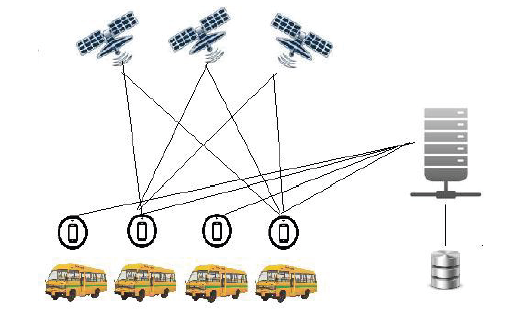
\includegraphics[width=0.6\columnwidth]{../figs/arch_mbts.png}
    \caption{Arquitetura do MBTS.}Fonte: \cite{sujatha}
    \label{fig:archMBTS}
\end{center}
\end{figure}

\newpage

Uma outra pesquisa neste área de acompanhamento de ônibus, envolve a utilização de \sigla{RF}{Radio frequência} (Radio frequência). Foi desenvolvida por \citeonline{paradells}.

Os autores propõe a utilização de uma rede de dados composta por transmissores e receptores RF. Os transmissores situam-se nos ônibus, os quais transmitem informações para os receptores, que situam-se nos pontos de ônibus que, basicamente, são os nós da rede. Assim que um ônibus se aproxima de um ponto de ônibus - nó - inicia a transmissão de informações relevantes, captadas por sensores atrelados ao veículo. Essas informações podem ser usadas/acessadas por um usuário que está aguardando no referido ponto de ônibus. 

Uma limitação do sistema baseado em RF, e percebida pelos próprios autores, diz respeito à distância entre o ônibus e os nós da rede (neste caso os pontos de ônibus). Uma vez que sensores baseados em radio frequência possuem limitações de distância e na transmissão dos dados, acabam limitando a velocidade desenvolvida pelo veículo, o que torna o projeto inviável. 

Ainda, as informações só podem ser coletadas por usuários que já estão próximos ao veículo (ou em pontos de ônibus próximos ao veículo). Isso acaba tirando o propósito de acompanhamento ou rastreio de ônibus, pois o mesmo já está próximo do ponto, e pode ser vislumbrado por um usuário sem o auxílio de um sistema específico para tal.

\citeonline{alves} apresentaram um sistema -- chamado de \emph{Trip-planner} -- para planejar rotas em tempo real, para pessoas que utilizam transporte público em Lisboa. O sistema consegue informar quais são as melhores rotas e o tempo estimado de viagem para um determinado destino, baseados na estimativa de quantos veículos estão trafegando e quais são suas velocidades.

Informações de tempo-real são coletadas através do GPS equipado nos ônibus. Essas informações são utilizadas em um servidor (o que os autores chamam de \emph{Data Center}) para atualizar históricos e melhorar as estimativas, uma vez que é utilizado um algoritmo para predição de tempos de viagem. Esses históricos se referem à relatórios de quatro meses, com informações sobre tempos de viagem e velocidades dos veículos. Essas informações são analisadas e passam por um classificador, e uma vez processadas, são repassadas para qualquer dispositivo móvel conectados em uma rede sem fio, através de \emph{broadcast} \cite{alves}.

\newpage

A Figura \ref{fig:archLisbon} descreve de forma simplificada o sistema proposto por \citeonline{alves}. Nota-se claramente que dados históricos e de tempo-real são coletados com o auxílio do GPS instalado no ônibus. Esses dados passam pelo \emph{Data Center} e são utilizados como entrada para um algoritmo de predição. Uma vez processados, distribuem-se os dados para dispositivos móveis através de \emph{broadcast.}

\begin{figure}[h]
\begin{center}
    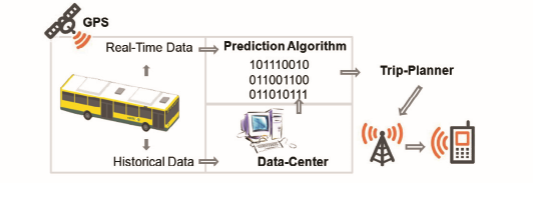
\includegraphics[width=0.85\columnwidth]{../figs/arch_lisbon.png}
    \caption{Arquitetura do \emph{Trip-planner}.}Fonte: \cite{alves}
    \label{fig:archLisbon}
\end{center}
\end{figure}